\documentclass[12pt,twocolumn]{article}
\usepackage{graphicx}
\usepackage{pdfpages}
\usepackage{hyperref}
\usepackage[margin=1.25in]{geometry}
\usepackage[utf8]{inputenc}
\graphicspath{ {./Figures/} }
\hypersetup{
    colorlinks=true,
    linkcolor=blue,
    filecolor=magenta,      
    urlcolor=cyan,
}
\urlstyle{same}
\usepackage[font={small,it}]{caption}
\usepackage{fancyvrb}
\title{Model \& Simulation of South Bend Government Call Center using Arena}
\author{John D. Bulger, Jacob D. White \& Adali J.J. Johnson\\Valparaiso University\thanks{``We have neither given or received, nor have we tolerated other’s use of unauthorized aid."}}
\date{October 23, 2018}

	\begin{document}
\maketitle

\section{Introduction}
The city of South Bend, located in northern Indiana, established a citizen-accessible call center in February 2013.  It addresses almost every aspect of city-citizen interaction, including waste pick-up and removal, water billing and disconnections, and code enforcement.  By serving as a central hub for communication, the call center is able to consolidate a substantial amount of data regarding citizens as consumers.  This data is available on South Bend's open data portal at \textit{https://data-southbend.opendata.arcgis.com}.

	\begin{figure}[h]
	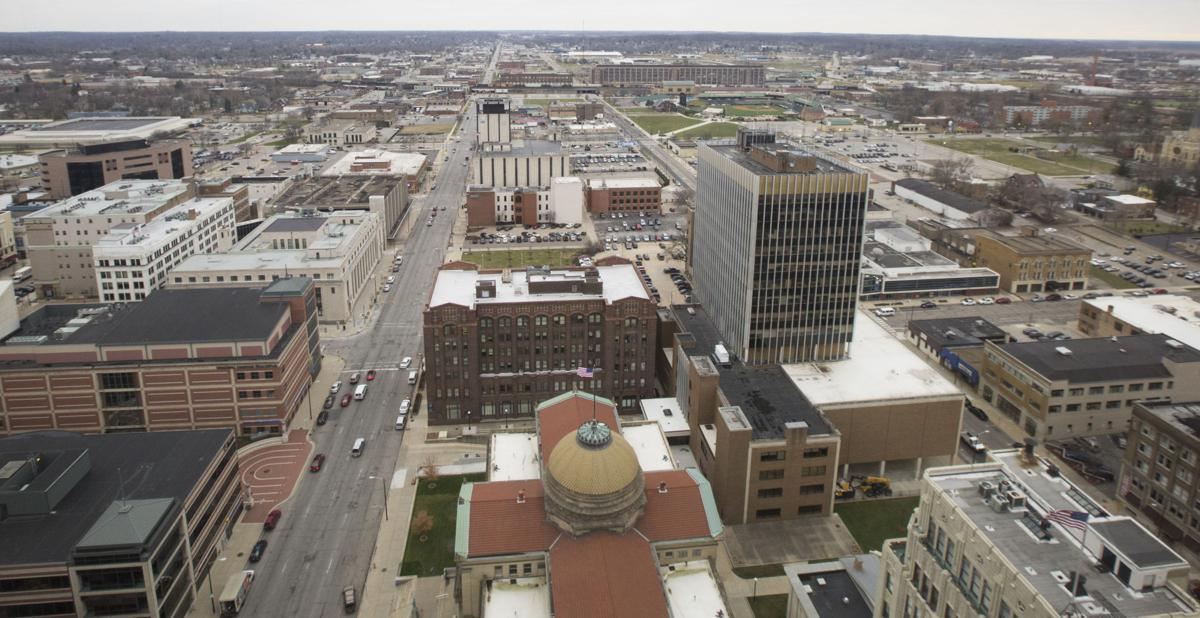
\includegraphics[scale=.17]{south_bend.png}
	\caption{South Bend, IN (Greg Swiercz)}
	\end{figure}

\par
The city's call center is seeking to explore XXXXX.  As such, this model and simulation will be constructed with the primary purpose of discovering an answer to this question in order to aid management's decision-making.  The call center will be modeled in Arena, as a discrete-event model, using the open-source data.  Through simulation, this question will be explored and answered.

\section{Background \& Terminology}
Call centers are a frequently studied topic within the simulation and modeling disciplines.  As such, some basic terminology shall be explained.  This model consists of two primary components:  calls and operators.  Calls will be represented as entities in Arena, as they are created and move through the system.  The operators, also known as ``311 liasons," will be represented as resources in Arena.

\par

For this exploration, an ``arrival" is defined as a unique call first coming into the call process model.



\section{Prior Work}

Call center and queuing analysis has been the focus of academic research for years.  Brown et al. provide an excellent overview of the Poisson distribution modeling customer arrivals, as well as the accompanying assumptions.  While arrival distribution is not analyzed in this paper, the authors' assumptions are, for the most part, assumed to be true in this analysis.  These center around the general assumption that the customers and operators are statistically identical and that they all act independently.\cite{brown}  Zhang, Hong, and Zhang also describe the arrival process as a Poisson distribution, but discuss models which may be more accurate alternatives.\cite{zhang}  They maintain some of the main assumptions as Brown.  As a result, differences in time-dependent parameters, customer attitudes and preferences, and operator skill levels are treated as negligible.
\par
Call centers are a prime opportunity to utilize simulation techniques.  In fact, according to Bapat and Pruitte, simulation is the preferred method to analyze and determine the effectiveness of a call center.\cite{bapat}  It allows for evaluation of metrics beyond what a basic analysis encompasses.  For example, the scheduling of call agents should be optimized against call duration and abandonment, as documented by Saltzman and Mehrota.\cite{saltzman}

\section{Mathematical Model}

Our core model structure is based off the work of Mandelbaun in 2001.  In his frequently referenced text, he lays out the basic schematic of a call center model.  His model illustrates the possible flow of a call starting with its arrival until disposal, be that as a lost call or having completed successfully.\cite{mandelbaun}  While simplistic by nature, the model covers all of the basic aspects of a call center in a sensible format that can easily by applied in Arena.  

	\begin{figure}[h]
	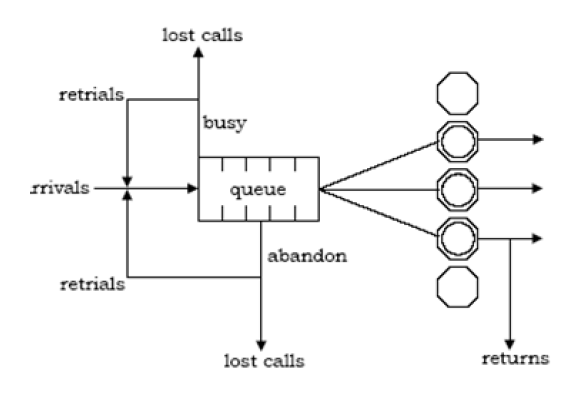
\includegraphics[scale=.45]{call_center_layout.png}
	\caption{Basic Operational Schematic of Call Center (Mandelbaun 2001)}
	\end{figure}


\subsection{Expanded Model}

% I need to rework all of this shit
While such arrivals are frequently defined with an exponential distribution, this model utilizes a more accurate representation of arrivals as calculated from the aforementioned open-source data.  

\par

While these calls move through the model, they will undergo several assignments, in which they are assigned a priority, language, and topic.  The topic will determine the duration distribution as identified from the open-source data, and the language (English or Spanish) will determine into which operator queue.  Calls will then enter a queue until they can speak to an agent.  After completing or abandoning the calls, the entity is referred to as ``disposed" since it leaves the model at that time.

	\begin{figure}[h]
	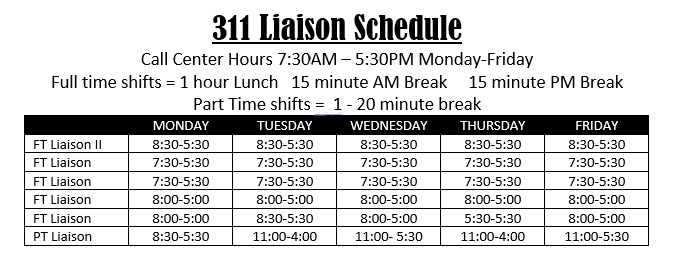
\includegraphics[scale=.35]{schedule2.jpg}
	\caption{Call center operator schedule}
	\end{figure}

\section{Simulation}



\section{Verification \& Validation}



\section{Results}



\section{Challenges}



\section{Discussion}



\begin{thebibliography}{7}
\bibitem{baraka}
Baraka, H., Baraka H. \& El-Gamily, I. (2013). Assessing call centers' success: A validation of the DeLone and Mclean model for information system. \textit{Egyptian Informatics Journal, 14}, 99-108.

\bibitem{brown}
Brown, L., Gans, N., Mandelbaum, A., Sakov, A., Shen, H., Zeltyn, S., \& Zhao, L. (2005). Statistical analysis of a telephone call center: a queueing-science perspective. \textit{Journal of the American Statistical Association, 100(469)}, 36-50.

\bibitem{zhang}
Xiaowei Zhang, L. Jeff Hong, \& Jiheng Zhang. (2014). Scaling and modeling of call center arrivals. \textit{In Proceedings of the 2014 Winter Simulation Conference (WSC '14)}. IEEE Press, Piscataway, NJ, USA, 476-485.

\bibitem{bapat}
Vivek Bapat \& Eddie B. Pruitte, Jr.. (1998). Using simulation in call centers. \textit{In Proceedings of the 30th conference on Winter simulation (WSC '98)}, D. J. Medeiros, Edward F. Watson, John S. Carson, and Mani S. Manivannan (Eds.). IEEE Computer Society Press, Los Alamitos, CA, USA, 1395-1400.

\bibitem{saltzman}
Robert Saltzman \& Vijay Mehrotra. (2007). Managing trade-offs in call center agent scheduling: methodology and case study. \textit{In Proceedings of the 2007 Summer Computer Simulation Conference (SCSC '07)}. Society for Computer Simulation International, San Diego, CA, USA, 643-651.

\bibitem{mandelbaun}
Mandelbaun A., A. Sakov and S. Zeltyn. 2001. Empirical Analysis of a Call Center. Technion Israel Institute of Technology, Israel.

\end{thebibliography}

\end{document}